%!LW recipe=latexmk-xelatex
\documentclass[compress]{beamer}

\usetheme[block=fill]{metropolis}

\usepackage{graphicx} % Allows including images
\usepackage{amsmath,amsfonts,amsthm,amssymb}
\usepackage{color}
\usepackage{xcolor,cancel}
\usepackage{tcolorbox}
\setbeamercolor{colorBoxStuff}{fg=black, bg=gray!30!white}
%\setitemize{label=\usebeamerfont*{itemize item}%
%	\usebeamercolor[fg]{itemize item}
%	\usebeamertemplate{itemize item}}
\definecolor{mDarkBrown}{HTML}{604c38}
\definecolor{mDarkTeal}{HTML}{23373b}
\definecolor{mLightBrown}{HTML}{EB811B}
\definecolor{mMediumBrown}{HTML}{C87A2F}
\definecolor{mygreen}{HTML}{98C2B9}
\definecolor{myyellow}{HTML}{DFD79C}
\definecolor{myblue}{HTML}{8CA7CC}
\definecolor{kern}{HTML}{8CC2B7}



\usepackage{float}
\usepackage{framed}
\usepackage{epsfig}
\usepackage{graphicx}
\usepackage{subcaption}
\usepackage{ulem}
\usepackage{hhline}
\usepackage{multirow}
\usepackage{comment}   
\usepackage{bbm}
\usepackage{tikz}   
\def\Put(#1,#2)#3{\leavevmode\makebox(0,0){\put(#1,#2){#3}}}
\newcommand*\mystrut[1]{\vrule width0pt height0pt depth#1\relax}
\newcommand{\eqdef}{\mathbin{\stackrel{\rm def}{=}}}


\newcommand{\bs}[1]{\boldsymbol{#1}}
\newcommand{\bv}[1]{\mathbf{#1}}
\newcommand{\R}{\mathbb{R}}
\newcommand{\E}{\mathbb{E}}

\DeclareMathOperator*{\argmin}{arg\,min}
\DeclareMathOperator*{\argmax}{arg\,max}
\DeclareMathOperator{\nnz}{nnz}
\DeclareMathOperator{\cut}{cut}
\DeclareMathOperator{\vol}{vol}
\DeclareMathOperator{\diag}{diag}
\DeclareMathOperator{\Var}{Var}
\DeclareMathOperator{\sinc}{sinc}
\DeclareMathOperator{\sign}{sign}
\DeclareMathOperator{\dist}{dist}
\DeclareMathOperator{\mv}{mv}
\DeclareMathOperator{\sgn}{sgn}
\DeclareMathOperator{\step}{step}
\DeclareMathOperator{\gap}{gap}
\DeclareMathOperator{\poly}{poly}
\DeclareMathOperator{\tr}{tr}
\DeclareMathOperator{\orth}{orth}
\newcommand{\norm}[1]{\|#1\|}
\captionsetup[subfigure]{labelformat=empty}
\captionsetup[figure]{labelformat=empty}
\DeclareMathOperator*{\lmin}{\lambda_{min}}
\DeclareMathOperator*{\lmax}{\lambda_{max}}

\newcommand{\specialcell}[2][c]{%
	\begin{tabular}[#1]{@{}c@{}}#2\end{tabular}}
\newcommand{\specialcellleft}[2][c]{%
	\begin{tabular}[#1]{@{}l@{}}#2\end{tabular}
}

\newtheorem{claim}[theorem]{Claim}
%\newtheorem{corollary}[theorem]{Corollary}

\usepackage{tabstackengine}
\stackMath


%----------------------------------------------------------------------------------------
%	TITLE PAGE
%----------------------------------------------------------------------------------------

\title{CS-GY 6763: Lecture 14 \\ Finish Sparse Recovery and Compressed Sensing, Introduction to Leverage Score Sampling}
\author{NYU Tandon School of Engineering, Prof. Christopher Musco}
\date{}

\begin{document}
	
	\begin{frame}
		\titlepage 
	\end{frame}
	
	\metroset{titleformat=smallcaps}
	
	\begin{frame}
	\frametitle{administrative}
	\textbf{This is our last class!}
		\begin{itemize}
			\item Final project due next Tuesday. 
			\item Exam study guide was released. Same rules as midterm (cheat sheet allowed). will be a 1.5 hour test.
			\item Solutions for last problem sets will be released tonight.
		\end{itemize}
	\end{frame}

	\begin{frame}
		\frametitle{course feedback}
		This course is taught every year and is now one of the primary ways of filling the theory breadth requirement for Ph.D. students, so it is important that we keep improving it. 

		\begin{center}
			
\includegraphics[width=.4\textwidth]{grad_qr_code.png}

			Graduate Section
		\end{center}
	\end{frame}


	\begin{frame}
		\frametitle{course feedback}
		\begin{center}
			
\includegraphics[width=.4\textwidth]{undergrad_qr_code.png}

			Undergraduate Section
		\end{center}
	\end{frame}

\begin{frame}
	\frametitle{sparsity recovery/compressed sensing}
	Design $\bv{A}\in\R^{m \times n}$ with $m < n$ rows so that we can recover $k$ sparse vector $\bv{x} \in \R^n$ from $\bv{b} = \bv{Ax}$. 
	\begin{center}
		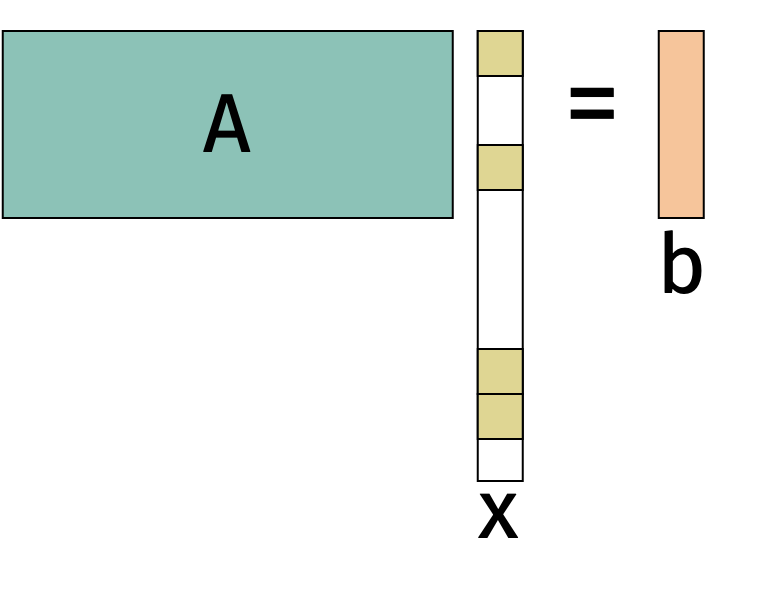
\includegraphics[width=.5\textwidth]{sparseRegressioon.png}
	\end{center}
\end{frame}
	
	\begin{frame}
		\frametitle{restricted isometry property}
		\begin{definition}[$(q,\epsilon)$-Restricted Isometry Property]
			A matrix $\bv{A}$ satisfies $(q,\epsilon)$-RIP if, for all $\bv{x}$ with $\|\bv{x}\|_0 \leq q$, 
			\begin{align*}
				(1-\epsilon)\|\bv{x}\|_2^2 \leq \|\bv{A}\bv{x}\|_2^2 \leq  (1+\epsilon)\|\bv{x}\|_2^2.
			\end{align*}
		\end{definition}
		Can argue this property holds for random JL matrice with $m = O\left(\frac{q\log (n/q)}{\epsilon^2}\right)$ rows. 
	\end{frame}

	\begin{frame}[t]
		\frametitle{restricted isometry property from jl}
		\begin{theorem}[Subspace Embedding from JL]
			Let $\mathcal{U} \subset \R^n$ be a $q$-dimensional linear subspace in $\R^n$. If $\bs{\Pi}\in \R^{m\times n}$ is chosen from any distribution $\mathcal{D}$ satisfying the Distributional  JL Lemma, then with probability $1-\delta$,
			\begin{align*}
				(1-\epsilon)\|\bv{v}\|_2^2 \leq \|\Pi \bv{v}\|_2^2 \leq	(1+\epsilon)\|\bv{v}\|_2^2
			\end{align*}
			for \emph{all} $\bv{v} \in \mathcal{U}$, as long as  $m = O\left(\frac{q + \log(1/\delta)}{\epsilon^2}\right)$.
		\end{theorem}		
		We will use union bound to apply this theorem to a collection of linear subspaces.
	\end{frame}

	\begin{frame}[t]
		\frametitle{restricted isometry property from jl}
		Let $\mathcal{S}_k = \{\bv{x}: \|\bv{x}\|_0 \leq q\}$ be the collection of all $q$ sparse vectors. 
		\begin{align*}
			\mathcal{S} = \mathcal{U}_1 \cup \ldots \cup \mathcal{U}_T,
		\end{align*}
		where $T = {n \choose q}$. 

	\end{frame}

	\begin{frame}[t]
		\frametitle{restricted isometry property from jl}
		\begin{theorem}[Subspace Embedding from JL]
			Let $\mathcal{U} \subset \R^n$ be a $q$-dimensional linear subspace in $\R^n$. If $\bs{\Pi}\in \R^{m\times n}$ is chosen from any distribution $\mathcal{D}$ satisfying the Distributional  JL Lemma, then with probability $1-\delta$,
			\begin{align*}
				(1-\epsilon)\|\bv{v}\|_2^2 \leq \|\Pi \bv{v}\|_2^2 \leq	(1+\epsilon)\|\bv{v}\|_2^2
			\end{align*}
			for \emph{all} $\bv{v} \in \mathcal{U}$, as long as  $m = O\left(\frac{q + \log(1/\delta)}{\epsilon^2}\right)$.
		\end{theorem}
		As long as we take a JL matrix with $O(\frac{q + \log(T)}{\epsilon^2})$ rows then it will preserve the norm of all vectors in $\mathcal{S} = \mathcal{U}_1 \cup \ldots \cup \mathcal{U}_T$ with high probability. 
		\begin{align*}
			\log(T) = \log {n \choose q} = \hspace{10em}
		\end{align*}
	\end{frame}


	\begin{frame}[t]
	\frametitle{first sparse recovery result}
	\begin{theorem}[$\ell_0$-minimization]
		Suppose we are given $\bv{A} \in \R^{m\times n}$ and $\bv{b} = \bv{A}\bv{x}$ for an unknown $k$-sparse $\bv{x} \in \R^n$.
		If $\bv{A}$ is $(2k,\epsilon)$-RIP for any $\epsilon < 1$ then $\bv{x}$ is the \emph{unique} minimizer of:
		\begin{align*}
			\min &\|\bv{z}\|_0 & &\text{subject to} & \bv{A}\bv{z} &= \bv{b} .
		\end{align*}
	\end{theorem}
\alert{\textbf{Problem:} This optimization problem naively takes $O(n^k)$ time to solve. }
\end{frame}
	
	\begin{frame}[t]
		\frametitle{polynomial time sparse recovery}
		\textbf{Convex relaxation of the $\ell_0$ minimization problem:}
		\begin{problem}[Basis Pursuit, i.e. $\ell_1$ minimization.]
			\begin{align*}
				\min_{\bv{z}} &\|\bv{z}\|_1 & &\text{subject to} & \bv{Az} &= \bv{b} .
			\end{align*}
		\end{problem}
		\begin{itemize}
			\item Objective is convex. \vspace{2em}
			
			\item Optimizing over convex set. 
		\end{itemize}
	Can be solved in $\poly(n)$ time using a linear program or using e.g. projected gradient descent. Other similar relaxations also work. E.g. Lasso regularization $\min_\bv{z} \|\bv{A}\bv{z} - \bv{b}\|_2 + \lambda \|\bv{z}\|_1$. 
	\end{frame}


	\begin{frame}[t]
	\frametitle{basis pursuit analysis}
	\begin{theorem}
		If $\bv{A}$ is $(3k, \epsilon)$-RIP for $\epsilon < .17$ and $\|\bv{x}\|_0 = k$, then $\bv{x}$ is the unique optimal solution of the Basis Pursuit optimization problem.
	\end{theorem}
	\textbf{Two surprising things about this result:}
	\begin{itemize}
		\item Exponentially improve computational complexity with only a \emph{constant factor} overhead in measurement complexity.
		\item Typical ``relax-and-round'' algorithm, but rounding is not even necessary! Just return the solution of the relaxed problem. 
	\end{itemize}
\begin{center}
	\textbf{\alert{Why $\ell_1$ norm instead of $\ell_2$ norm?}}
\end{center}
\end{frame}
	
	\begin{frame}[t]
		\frametitle{basis pursuit intuition}
		Suppose $\bv{A}$ is $2\times 1$, so $\bv{b}$ is just a scalar and $\bv{x}$ is a 2-dimensional vector.
		\begin{figure}[h]
			\centering
			\begin{subfigure}[t]{0.48\textwidth}
				\centering
				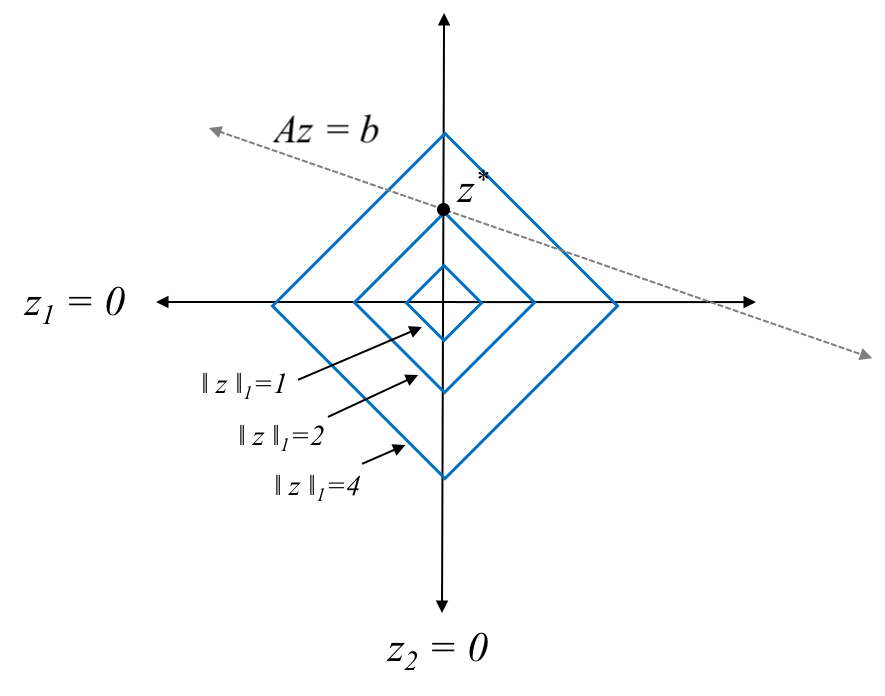
\includegraphics[width=\textwidth]{l1opt.png}
				\caption{Vertices of level sets of $\ell_1$ norm correspond to sparse solutions.}
			\end{subfigure}
			~
			\begin{subfigure}[t]{0.48\textwidth}
				\centering
				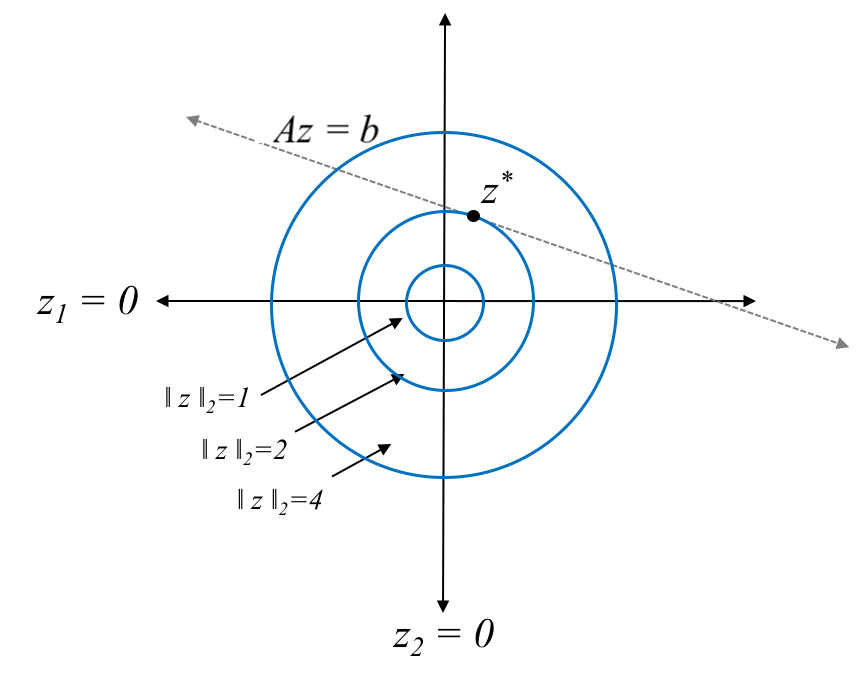
\includegraphics[width=\textwidth]{l2opt.png}
				\caption{This is not the case e.g. for the $\ell_2$ norm.}
			\end{subfigure}
		\end{figure}
		\vspace{-.5em}
		\begin{align*}
			\min_{\bv{z}} &\|\bv{z}\|_1 & &\text{subject to} & \bv{Az} &= \bv{b} .
		\end{align*}
	\end{frame}
	
	\begin{frame}[t]
		\frametitle{basis pursuit analysis}
		\begin{theorem}
			If $\bv{A}$ is $(3k, \epsilon)$-RIP for $\epsilon < .17$ and $\|\bv{x}\|_0 = k$, then $\bv{x}$ is the unique optimal solution of the Basis Pursuit LP).
		\end{theorem}
		\text{Similar proof to $\ell_0$ minimization:}
		\begin{itemize}
			\item By way of contradiction, assume $\bv{x}$ is \emph{not the optimal solution}. Then there exists some non-zero ${\Delta}$ such that:
			\begin{itemize}
				\item $\|\bv{x} + {\Delta}\|_1 \leq \|\bv{x}\|_1$
				\item $\bv{A}(\bv{x} + {\Delta}) = \bv{A}\bv{x}$. I.e. $\bv{A}{\Delta} = 0$.
			\end{itemize}
		\end{itemize}
		Difference is that we can no longer assume that $\Delta$ is sparse. 
		
		\begin{center}
			\alert{We will argue that $\Delta$ is ``approximately'' sparse.} 
		\end{center}
	\end{frame}
	
	\begin{frame}[t]
		\frametitle{tools needed}		
		\textbf{First tool:}
		\begin{align*}
			\text{For any $q$-sparse vector } &\bv{w}, & \|\bv{w} \|_2 \leq \|\bv{w} \|_1 \leq \sqrt{q}\|\bv{w}\|_2
		\end{align*}
		\vspace{3em}
		
		\textbf{Second tool:}
		\begin{align*}
			\text{For any norm and vectors $\bv{a},\bv{b}$, }& & \|\bv{a}+ \bv{b}\| \geq \|\bv{a}\| - \|\bv{b}\|
		\end{align*}
		
		
	\end{frame}
	
	\begin{frame}[t]
		\frametitle{basis pursuit analysis}\small
		\textbf{Some definitions:} $S$ is the set of $k$ non-zero indices in $\bv{x}$. $\bar{T}_1$ is the set of $2k$ indices \emph{not in $S$} with largest magnitude in $\Delta$. $\bar{T}_2$ is the set of $2k$ indices  \emph{not in $S$} with next largest magnitudes, etc.
		\begin{center}
			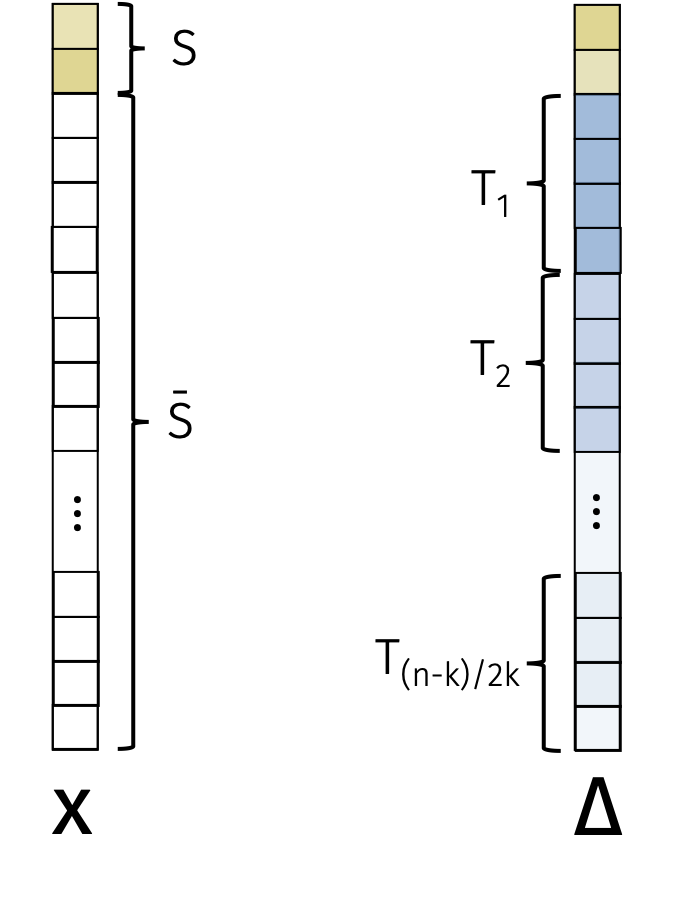
\includegraphics[width=.45\textwidth]{indexingForProof.png}
		\end{center}
		$T_1$ contains the $2k$ indices with largest value in $\Delta$ \emph{that are zero in $\bv{x}$}. $T_2$ contains the next $2k$ largest entries, etc. 
	\end{frame}
	
	\begin{frame}[t]
		\frametitle{basis pursuit analysis}
		\textbf{Recall:} By way of contradiction, if $\bv{x}$ is not the minimizer of the $\ell_1$ problem, then there is some $\Delta$ such that $\bv{A}(\bv{x} + \Delta) = \bv{b}$ and $\|\bv{x} + \Delta\|_1 \leq \|\bv{x}\|_1$.
		
		\vspace{1em} 
		\textbf{Claim 1 (approximate sparsity of $\Delta$):}
		$\|\Delta_{S}\|_1 \geq \|\Delta_{\bar{S}}\|_1$
	\end{frame}
	
	\begin{frame}[t]
		\frametitle{basis pursuit analysis}
		\textbf{Claim 2 ($\ell_2$ approximate sparsity):}
		$\|\Delta_{S}\|_2 \geq \sqrt{2}\sum_{j\geq 2} \|\Delta_{T_j}\|_2$:
		
		We have:
		\begin{align*}
			\|\Delta_s\|_2 \geq \frac{1}{\sqrt{k}} \|\Delta_{S}\|_1 \geq \frac{1}{\sqrt{k}}\|\Delta_{\bar{S}}\|_1 = \frac{1}{\sqrt{k}}\sum_{j\geq 1} \|\Delta_{T_j}\|_1.
		\end{align*}
		
		So it suffices to show that: $\|\Delta_{T_j}\|_1 \geq \sqrt{2k}\|\Delta_{T_{j+1}}\|_2$
	\end{frame}
	
	\begin{frame}[t]
		\frametitle{basis pursuit analysis}
		\textbf{Finish up proof by contradiction:}
		Recall that $\bv{A}$ is assumed to have the $(3k,\epsilon)$ RIP property. And by way of contradiction $\bv{A}(\bv{x} + \Delta) = \bv{b}$.
		\begin{align*}
			0 = \|\bv{A}\Delta\|_2 \geq  \|\bv{A}\Delta_{S\cup T_1}\|_2 - \sum_{j\geq 2} \|\bv{A}\Delta_{T_j}\|_2
		\end{align*}
	\end{frame}

	\begin{frame}[t]
	\frametitle{basis pursuit analysis}
	We have that $(1-\epsilon) - \frac{1+\epsilon}{\sqrt{2}} \geq 0$ whenever $\epsilon < .17$.
		\begin{center}
			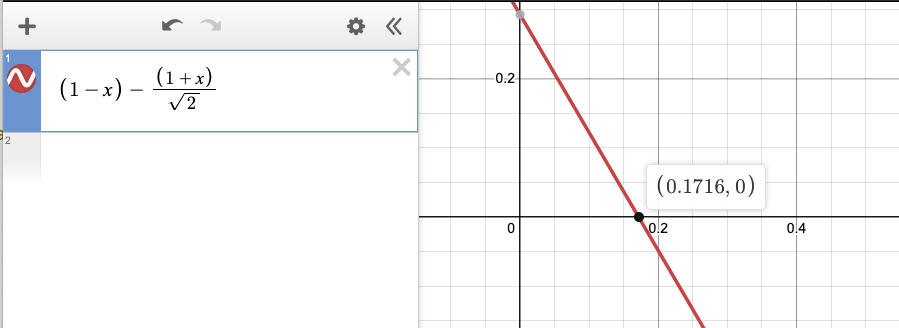
\includegraphics[width=.8\textwidth]{desmos.png}
		\end{center}
		\begin{theorem}
		If $\bv{A}$ is $(3k, \epsilon)$-RIP for $\epsilon < .17$ and $\|\bv{x}\|_0 = k$, then $\bv{x}$ is the unique optimal solution of the Basis Pursuit optimization problem, which can be solved in polynomial time.
	\end{theorem}
	\end{frame}
	
	\begin{frame}
		\frametitle{faster methods}
		A lot of interest in developing even faster algorithms that avoid using the ``heavy hammer'' of linear programming, which runs in roughly $O(n^{3.5})$ time. 
		
		\begin{itemize}
			\item \textbf{Iterative Hard Thresholding}: Looks a lot like projected gradient descent. Solve $\min_{\bv{z}} \|\bv{Az} - \bv{b}\|$ with gradient descent while continually projecting $z$ back to the set of $k$-sparse vectors. Runs in time \alert{$\sim O(n k\log n)$} for Gaussian measurement matrices and \alert{$O(n\log n)$} for subsampled Fourer matrices.
			\item Other ``first order'' type methods: Orthogonal Matching Pursuit, CoSaMP, Subspace Pursuit, etc.
		\end{itemize}
		
		%	One example of such an algorithm is Iterative Hard Thresholding \cite{iht}, which looks a lot like the projected gradient descent method we saw in class. The idea is to solve $\min_z \|z - Ax\|$ via a gradient method, . While this set is \emph{not convex} it's possible to show that the method still converges very rapidly. See \url{http://people.seas.harvard.edu/~minilek/cs229r/fall13/lec/lec18.pdf} for an analysis. The runtime of the method is approximately $O(n k\log n)$ for Gaussian measurement matrices and $O(n\log n)$ for subsampled Fourier matrices. Other ``first order'' type methods obtain similar running times. If you are interested in learning more, some algorithms to look up include ``Orthogonal Matching Pursuit'', "CoSaMP", and ``Subspace Pursuit''.
	\end{frame}
	
	\begin{frame}
		\frametitle{faster methods}
		When $\bv{A}$ is a subsampled Fourier matrix, there are now methods that run in \alert{\emph{$O(k\log^c n)$}} time [Hassanieh, Indyk, Kapralov, Katabi, Price, Shi, etc. 2012+].
		
		\begin{center}
			\textbf{Wait a minute...}
		\end{center}
		
	\end{frame}
	
	\begin{frame}
		\frametitle{sparse fourier transform}
		\textbf{Corollary:} When $\bv{x}$ is $k$-sparse, we can compute the inverse Fourier transform $\bv{F}^*\bv{F}\bv{x}$ of $\bv{F}\bv{x}$ in $O(k\log^c n)$ time!
		\begin{itemize}
			\item Randomly subsample $\bv{F}\bv{x}$.
			\item Feed that input into our sparse recovery algorithm to extract $\bv{x}$. 
		\end{itemize}
		\begin{center}
			\alert{Fourier and inverse Fourier transforms in \emph{sublinear time} when the output is sparse. }
			
			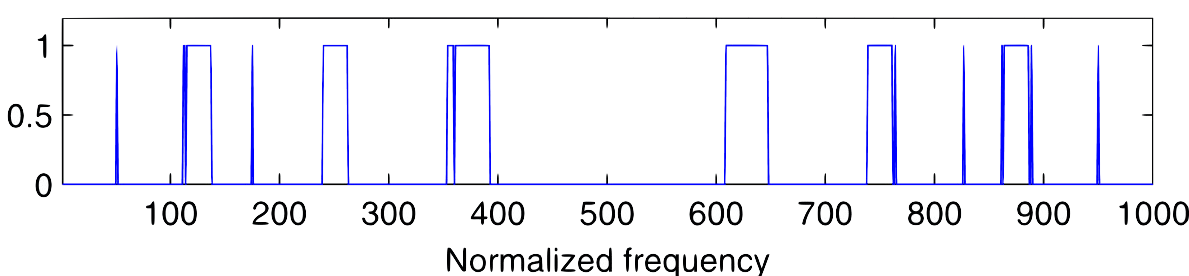
\includegraphics[width=.8\textwidth]{multiband.png}
		\end{center}
		\textbf{Applications in:} Wireless communications, GPS, protein imaging, radio astronomy, etc. etc. 
	\end{frame}

\begin{frame}
	\frametitle{compressed sensing for images}
	Compressed sensing for image data is based on the idea that ``natural images'' are sparse if \emph{some basis}. E.g. the DCT or Wavelet basis.
	
		\begin{center}
		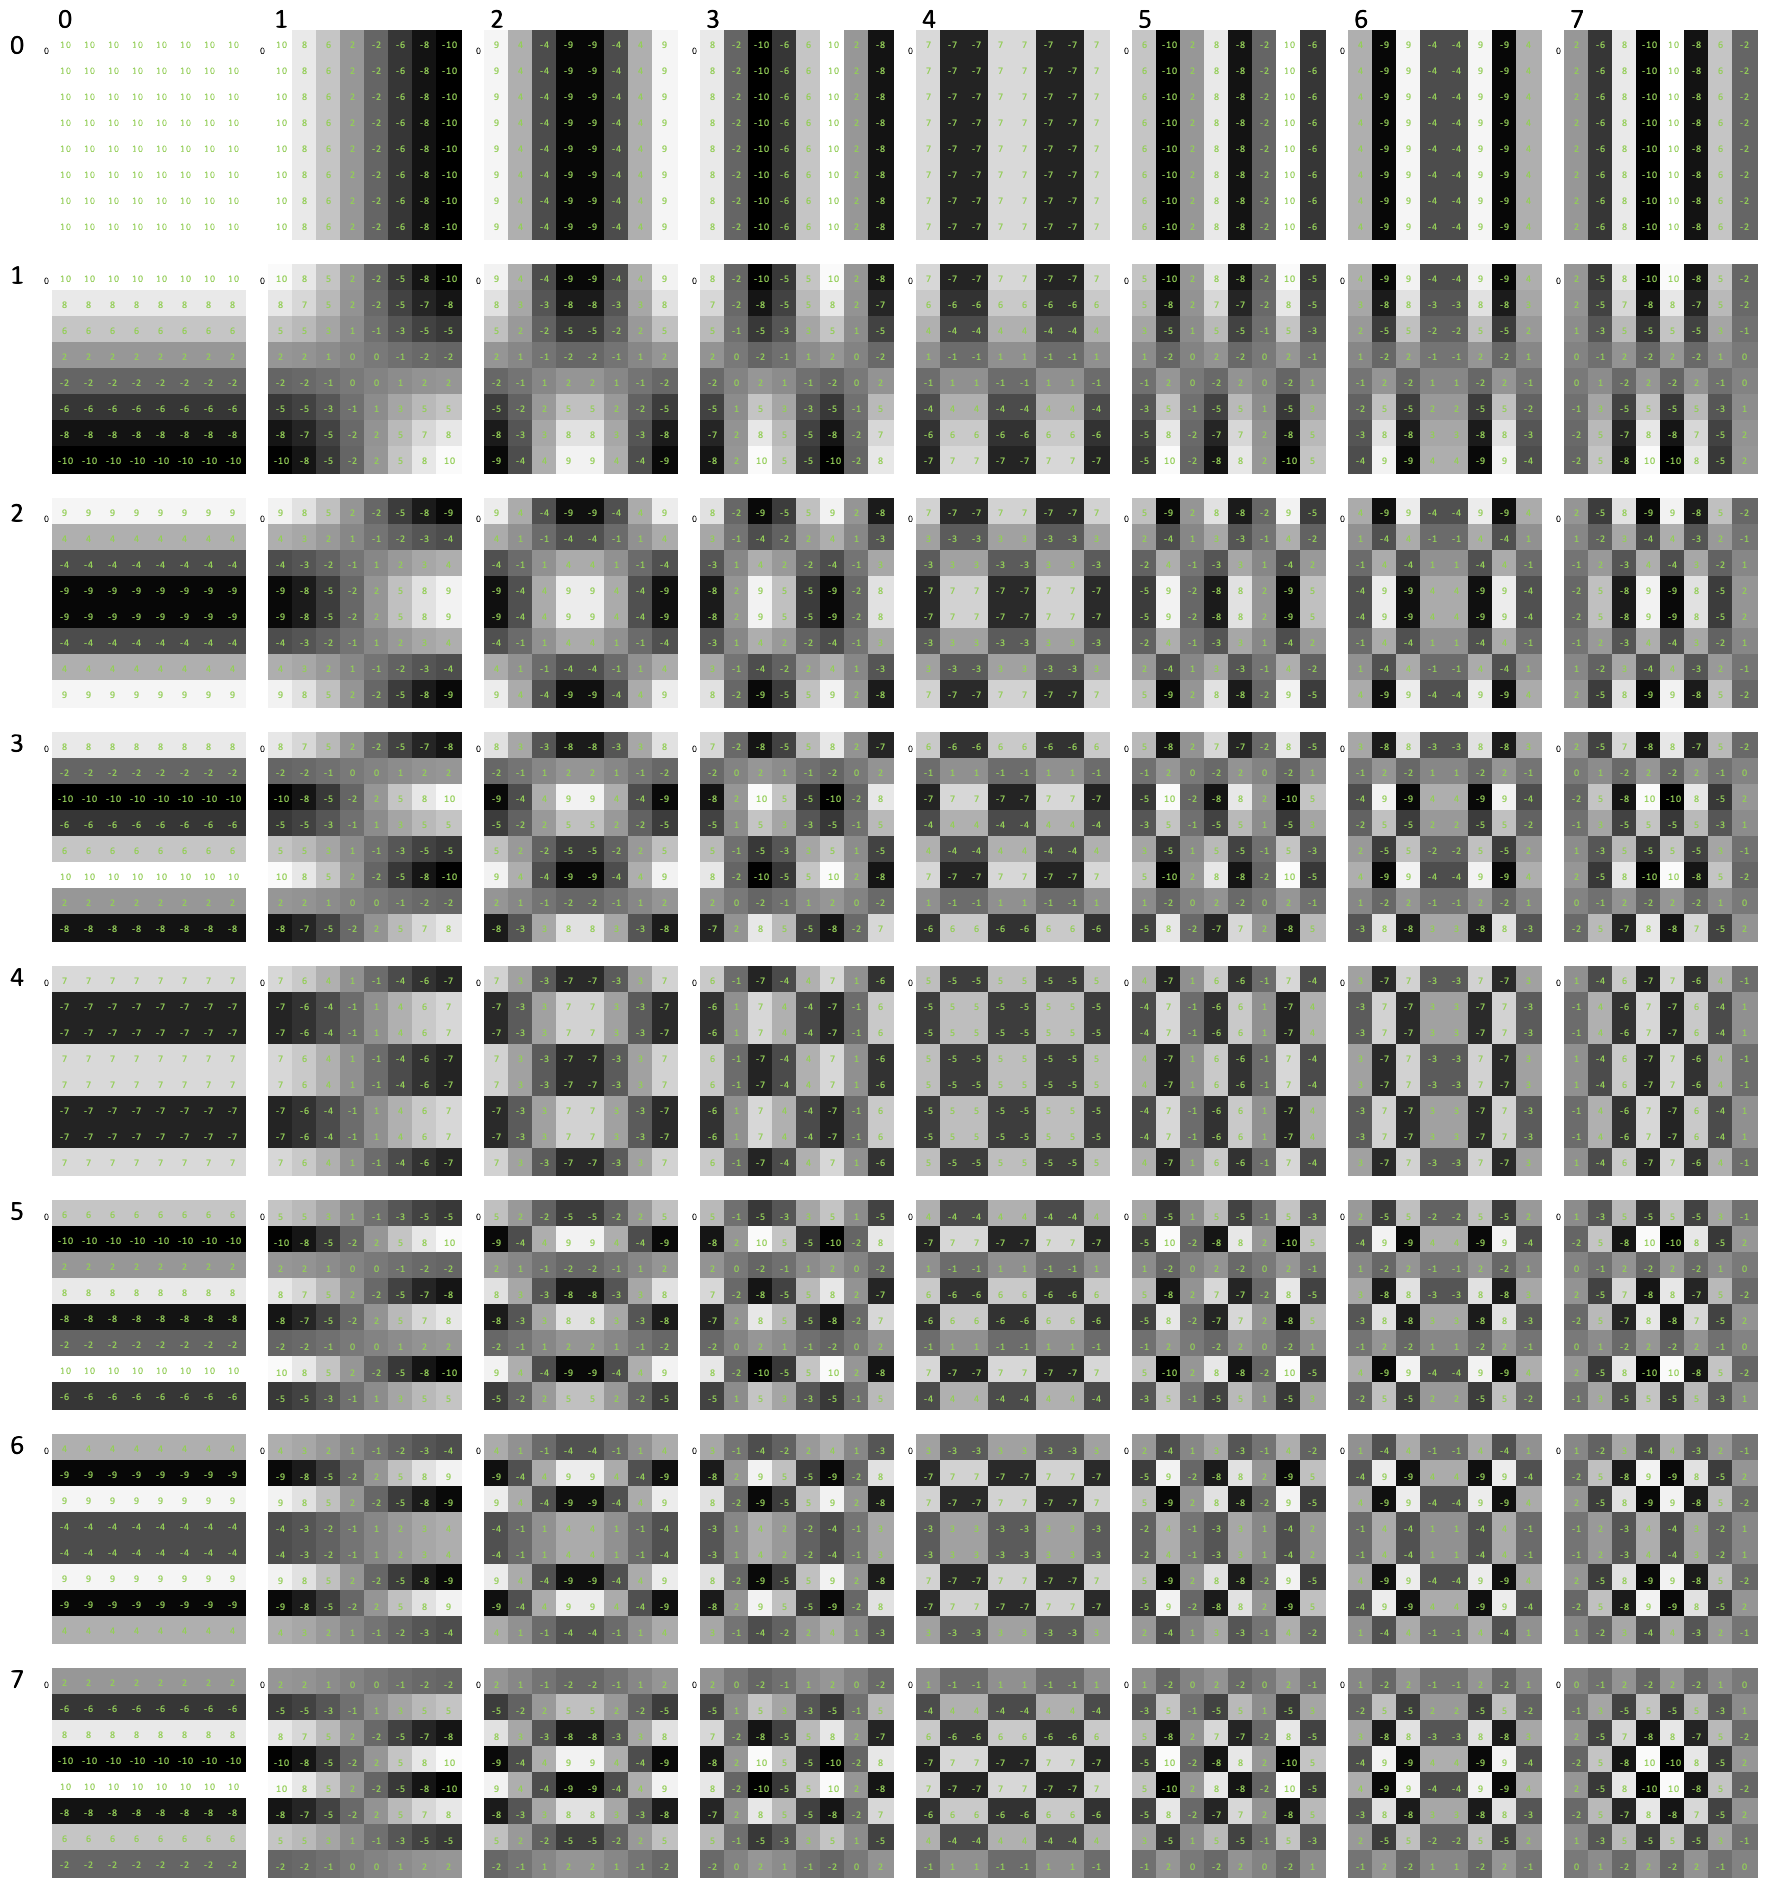
\includegraphics[width=.33\textwidth]{dct.png}		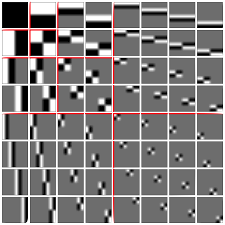
\includegraphics[width=.35\textwidth]{wavelet.png}
		\end{center}
	
	I.e. there is some representation of the image that requires many fewer numbers than explicitly writing down the pixels. 
\end{frame}

\begin{frame}
	\frametitle{compressed sensing related to modern deep learning method methods}
	\begin{center}
		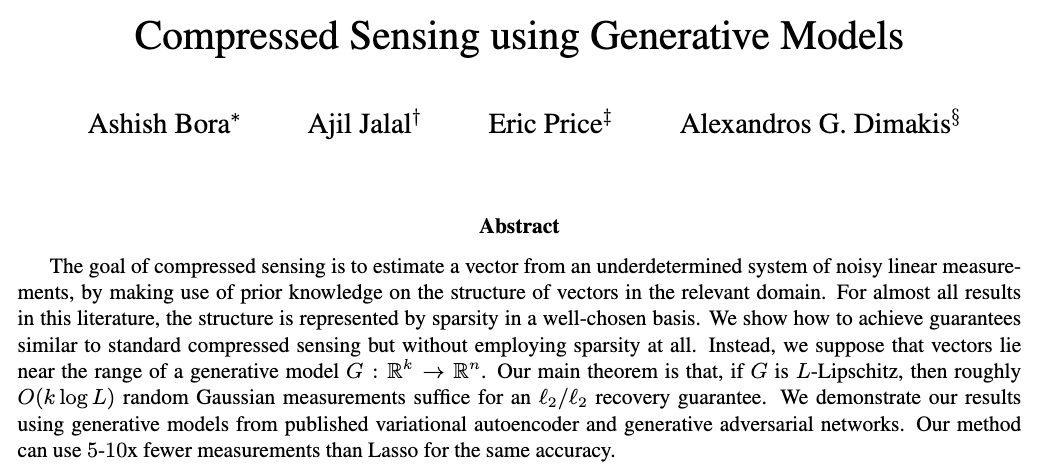
\includegraphics[width=.7\textwidth]{price1.png}
		
		\vspace{.5em}
		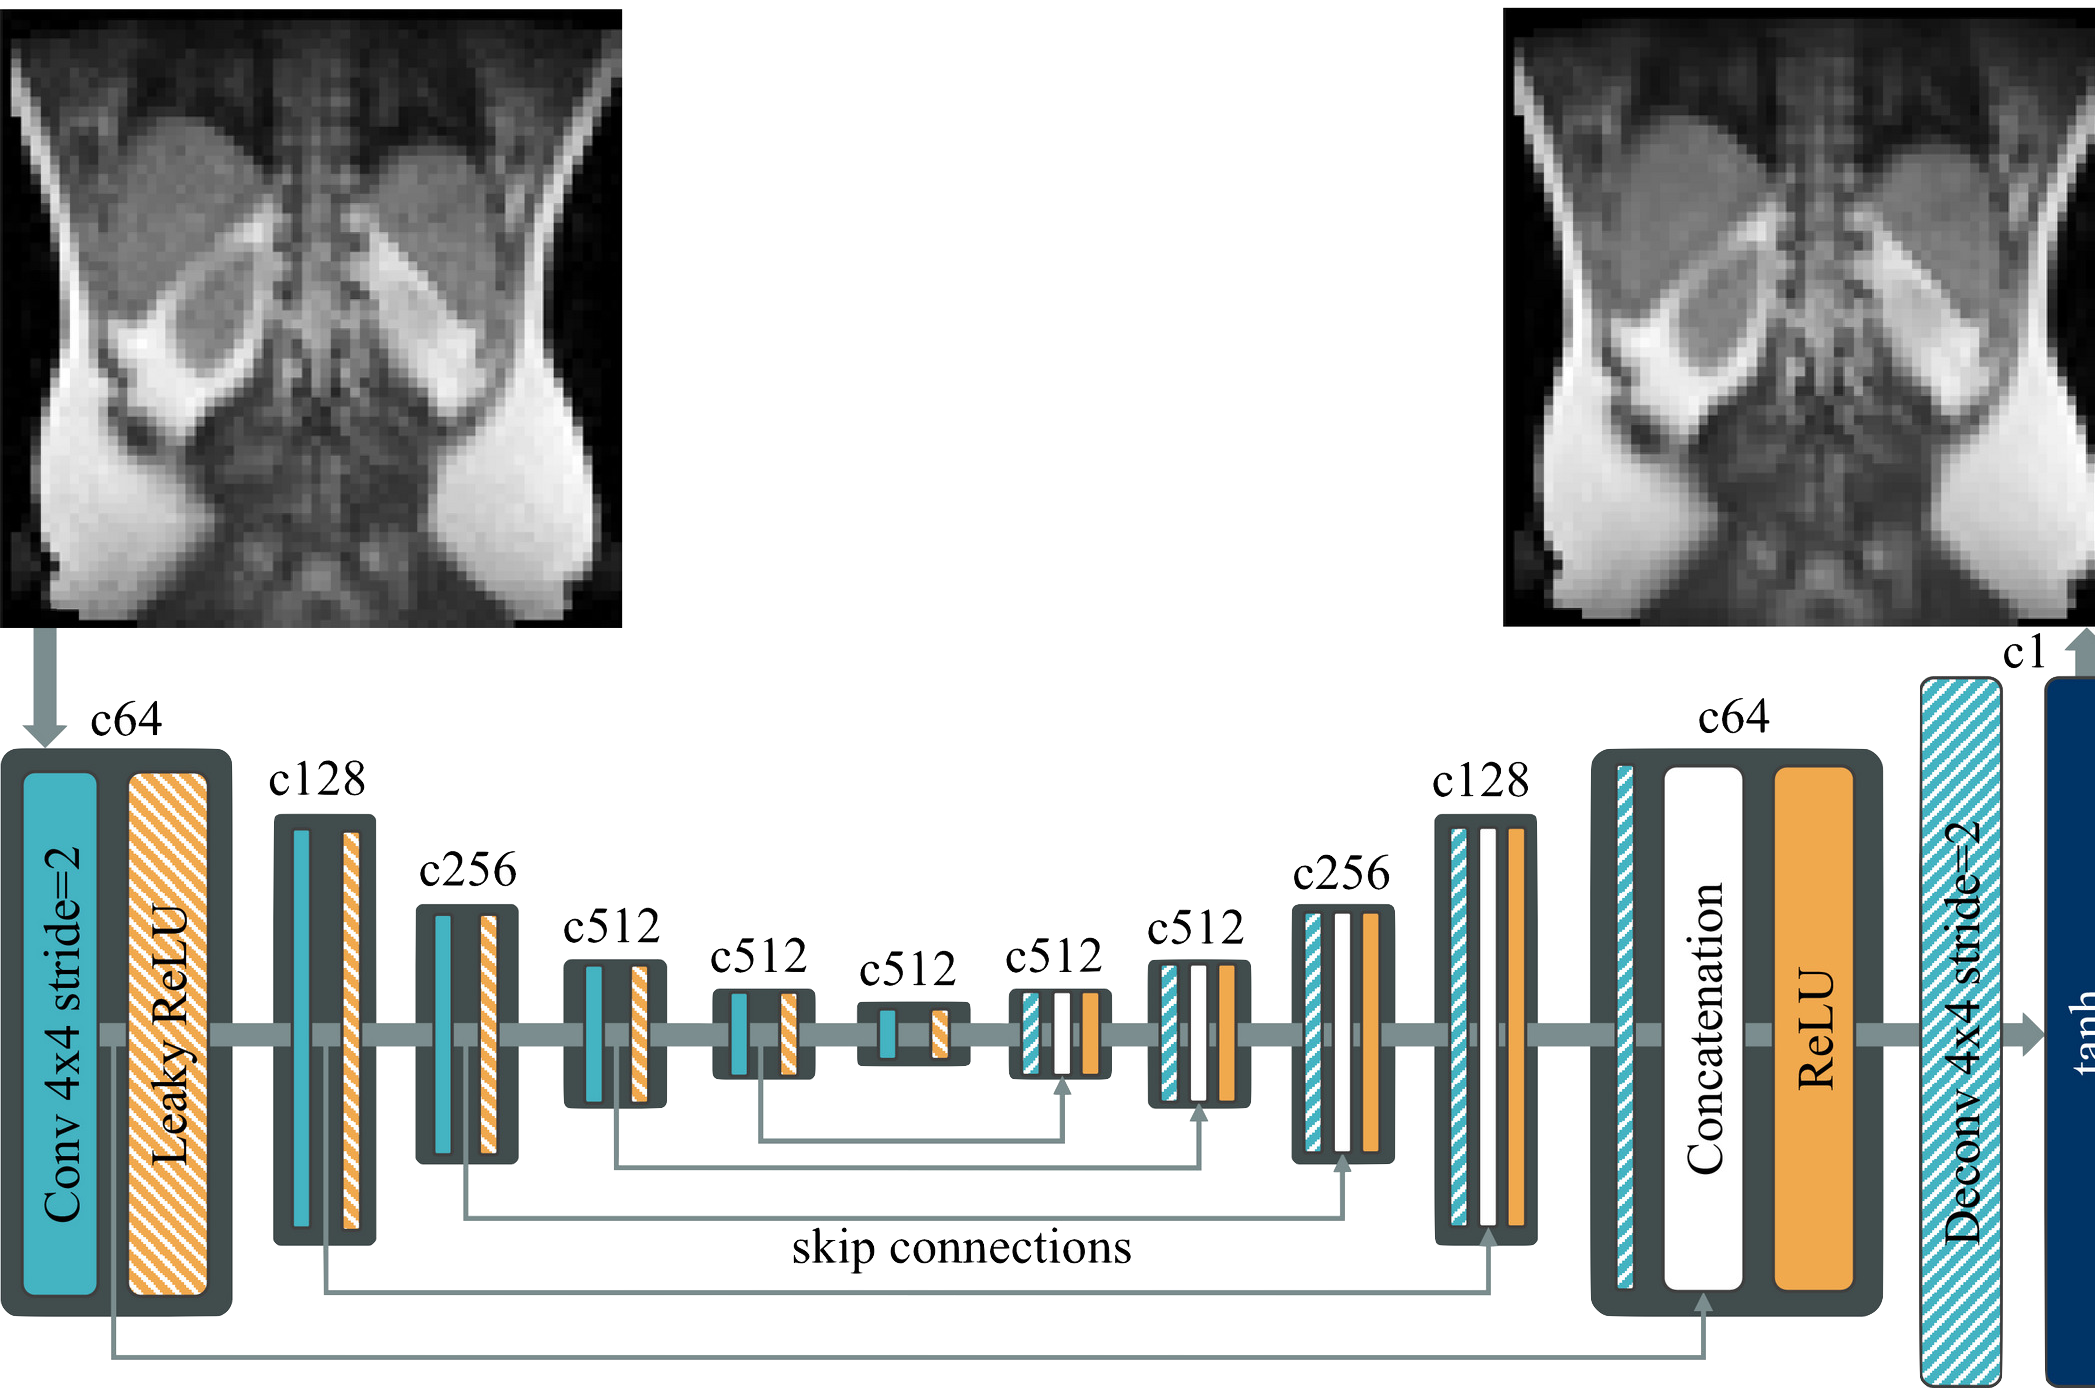
\includegraphics[width=.5\textwidth]{medical_autoencode.png}
	\end{center}
\end{frame}

\begin{frame}
	\frametitle{compressed sensing from generative models}
	For most generative models (e.g., GANs) output is parameterized by a short seed vector $\bv{z}$. 
	\vspace{-.5em}
	\begin{center}
		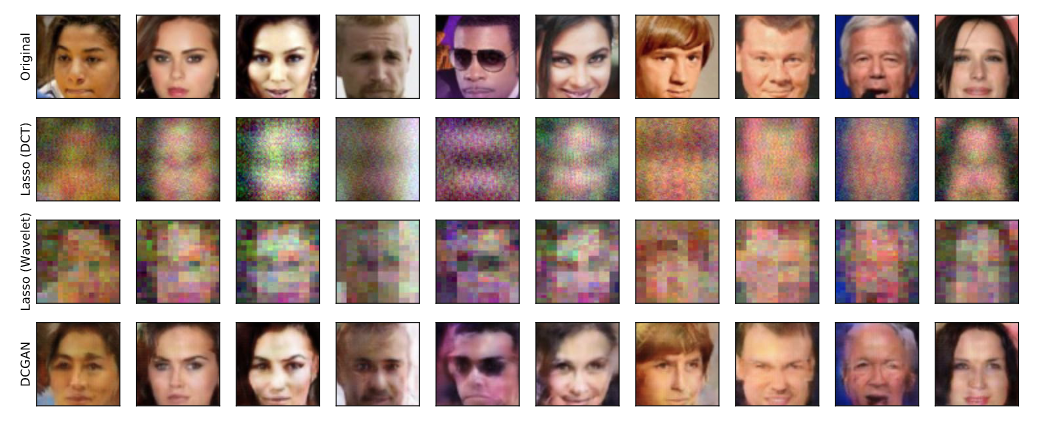
\includegraphics[width=\textwidth]{price2.png}
	\end{center}
	\vspace{-1em}

\textbf{Process:} measure image $\bv{x}$ by computing $\bv{b} = \bv{A}\bv{x}$ for a random matrix $\bv{A}$. Use gradient descent to find $\bv{z}\in \R^k$ to minimize:
\begin{align*}
	\|\bv{A}\mathcal{G}(\bv{z}) - \bv{b}\|.
\end{align*}
Return $\mathcal{G}(\bv{z})$. 
\end{frame}


\begin{frame}[standout]
	\begin{center}
		\large a little about my research
	\end{center}
\end{frame}

\begin{frame}
	\frametitle{subspace embeddings reworded}
	\begin{theorem}[Subspace Embedding]
		Let $\bv{A} \in \R^{n\times d}$ be a matrix. If $\bs{\Pi}\in \R^{m\times n}$ is chosen from any distribution $\mathcal{D}$ satisfying the Distributional JL Lemma, then with probability $1-\delta$,
		\begin{align*}
			(1-\epsilon)\|\bv{A}\bv{x}\|_2^2 \leq \|\bs{\Pi} \bv{A} \bv{x}\|_2^2 \leq	(1+\epsilon)\|\bv{A}\bv{x}\|_2^2
		\end{align*}
		for \emph{all} $\bv{x} \in \R^d$, as long as  $m = {O}\left(\frac{d + \log(1/\delta)}{\epsilon^2}\right)$.
	\end{theorem}
	Implies regression result, and more. 
	
	\textbf{Example:} Any singular value $\tilde{\sigma}_i$ of $\bs{\Pi}\bv{A}$ is a $(1\pm \epsilon)$ approximation to the true singular value ${\sigma}_i$ of  $\bv{B}$. 
\end{frame}

\begin{frame}
	\frametitle{subsampling methods}
	\begin{center}
		\textbf{Recurring research interest:} Replace random projection methods with \emph{random sampling methods}. Prove that for essentially all problems of interest, can obtain same asymptotic runtimes. 
		
		\vspace{.5em}
		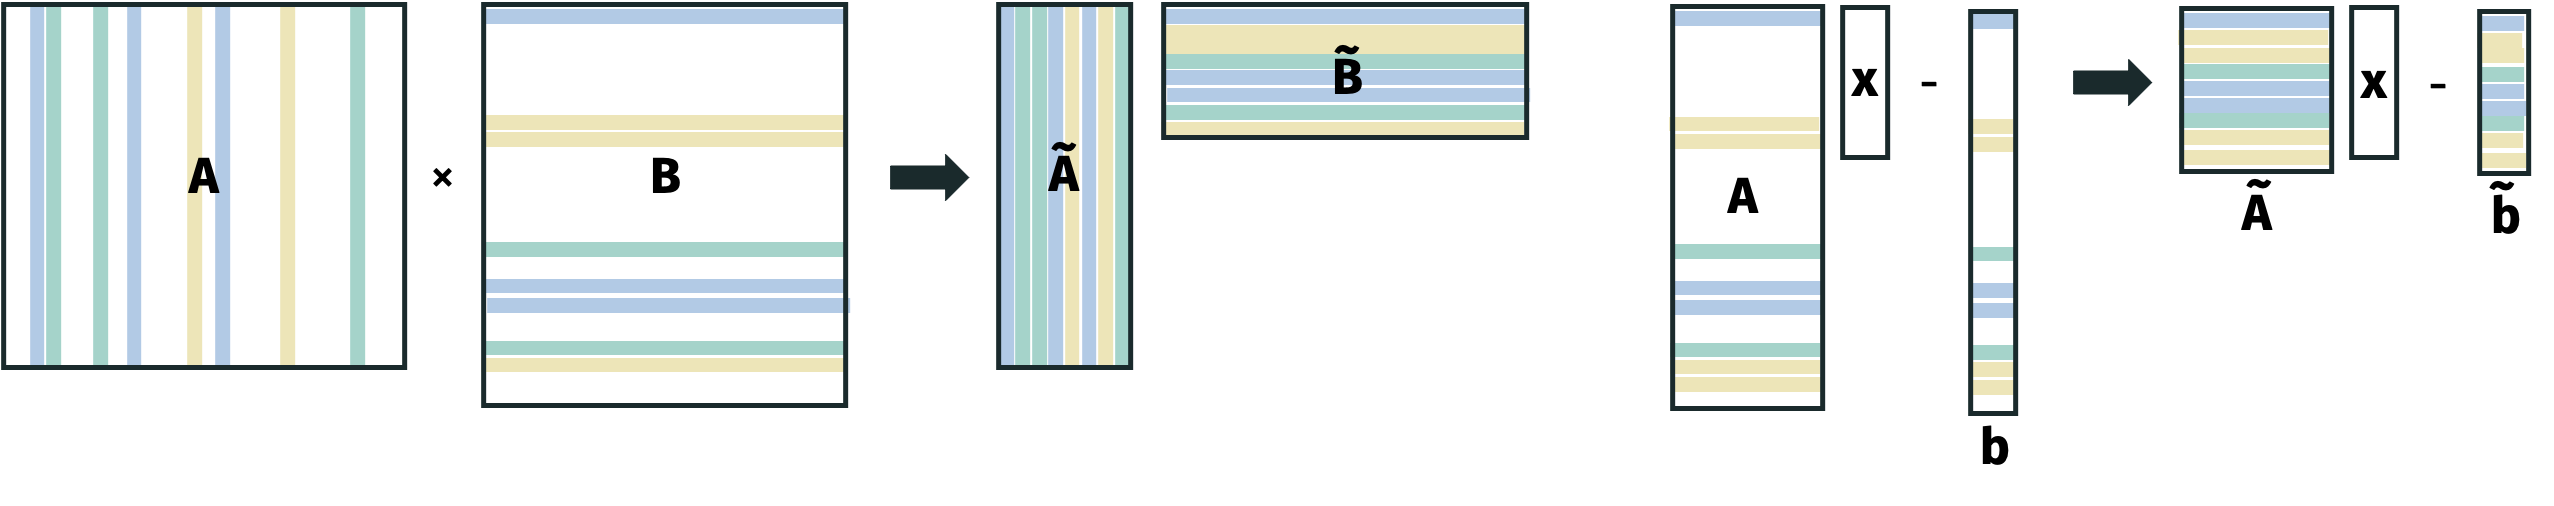
\includegraphics[width=\textwidth]{subsampling_high_level.png}
		
		Sampling has the added benefit of \emph{preserving matrix sparsity or structure}, and can be applied in a \emph{wider variety of settings} where random projections are too expensive.
	\end{center}
\end{frame}


\begin{frame}
	\frametitle{subsampling methods}
	\textbf{Goal:} Can we use sampling to obtain subspace embeddings? I.e. for a given $\bv{A}$ find $\tilde{\bv{A}}$ whose rows are a (weighted) subset of rows in $\bv{A}$ and:
	\begin{align*}
		(1-\epsilon)\|\bv{A}\bv{x}\|_2^2 \leq \|\tilde{\bv{A}}\bv{x}\|_2^2 \leq (1+\epsilon)\|\bv{A}\bv{x}\|_2^2.
	\end{align*}
	\begin{center}
		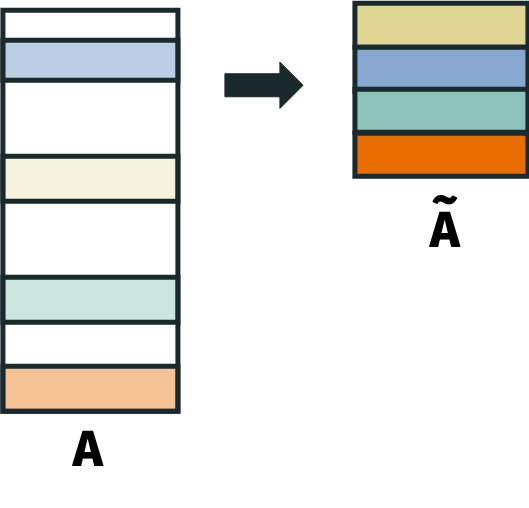
\includegraphics[width=.4\textwidth]{subsampleA.png}
	\end{center}
	
	
\end{frame}

\begin{frame}
	\frametitle{example where structure matters}
	Let $\bv{B}$ be the edge-vertex incidence matrix of a graph $G$ with vertex set $V$, $|V| = d$. Recall that $\bv{B}^T\bv{B} = \bv{L}$.
	\begin{center}
		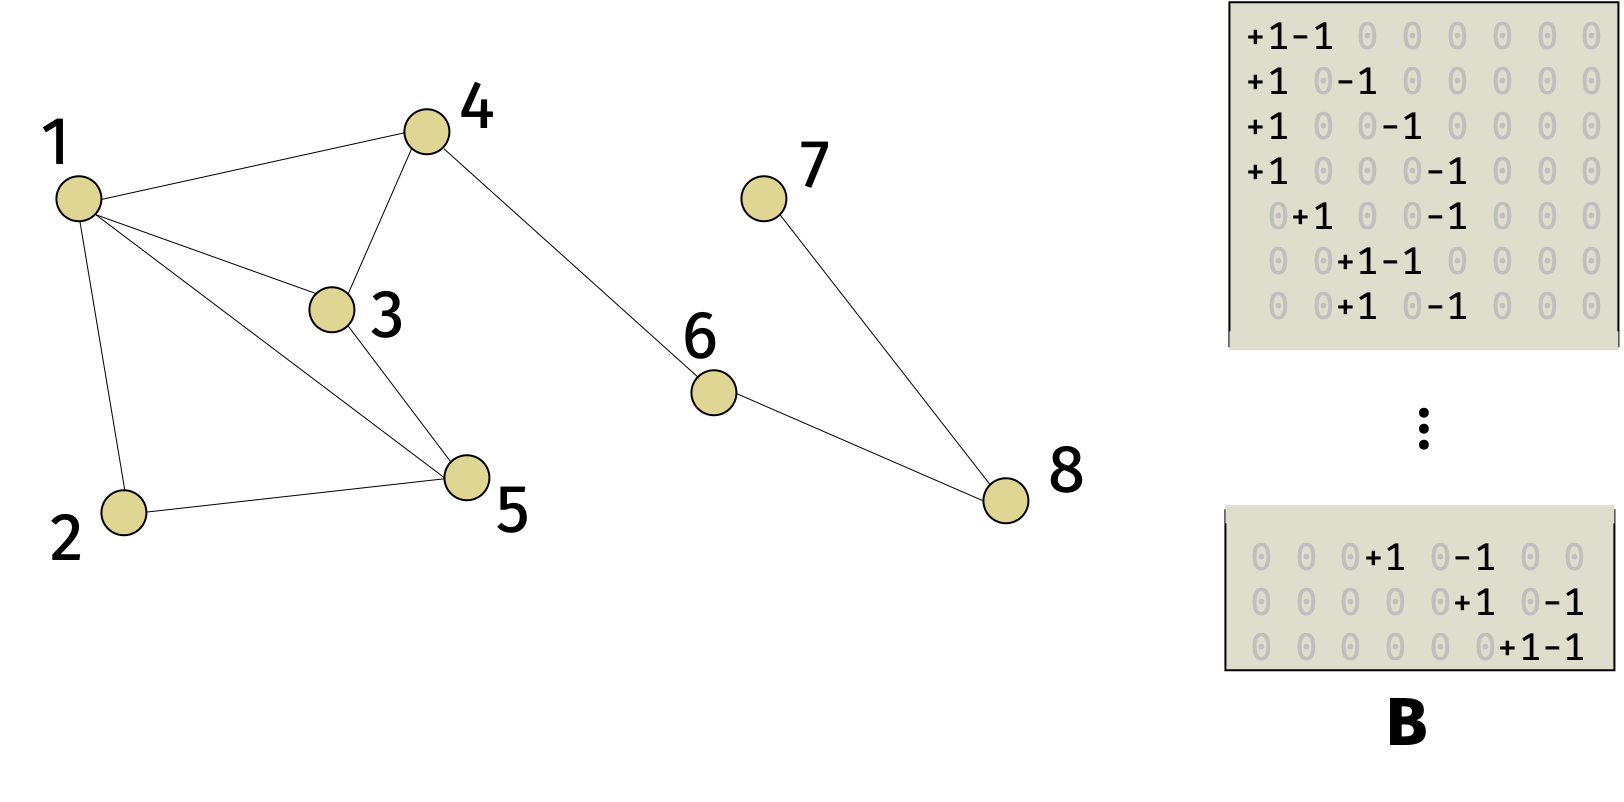
\includegraphics[width=\textwidth]{edge_vertex.png}
	\end{center}
	\vspace{-1em}
	
	Recall that if $\bv{x}\in \{-1,1\}^n$ is the \emph{cut indicator vector} for a cut $S$ in the graph, then $\frac{1}{4}\|\bv{B}\bv{x}\|_2^2 = \cut(S,V\setminus S)$.	
\end{frame}

\begin{frame}
	\frametitle{linear algebraic view of cuts}
	\begin{align*}
		\bv{x} = [1,1,1,-1,1,-1,-1,-1]
	\end{align*}
	\begin{center}
		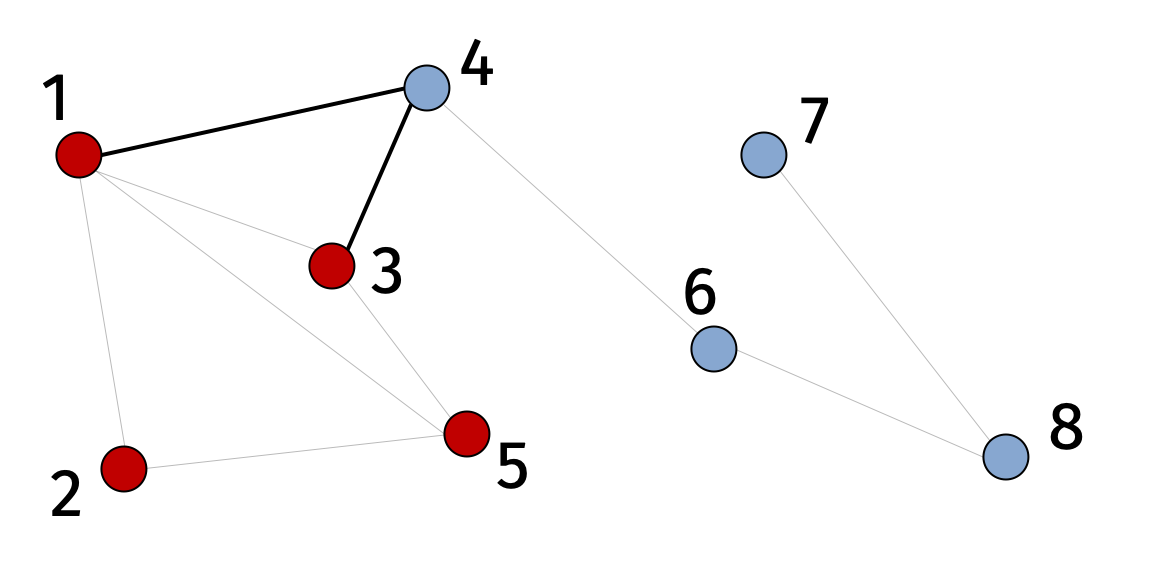
\includegraphics[width=.8\textwidth]{cut_example.png}
	\end{center}
	\vspace{-1em}
	$\bv{x}\in \{-1,1\}^d$ is the \emph{cut indicator vector} for a cut $S$ in the graph, then $\frac{1}{4}\|\bv{B}\bv{x}\|_2^2 = \cut(S,V\setminus S)$	
\end{frame}

\begin{frame}
	\frametitle{weighted cuts}
	Extends to weighted graphs, as long as square root of weights is included in $\bv{B}$. Still have the $\bv{B}^T\bv{B} = \bv{L}$.
	\begin{center}
		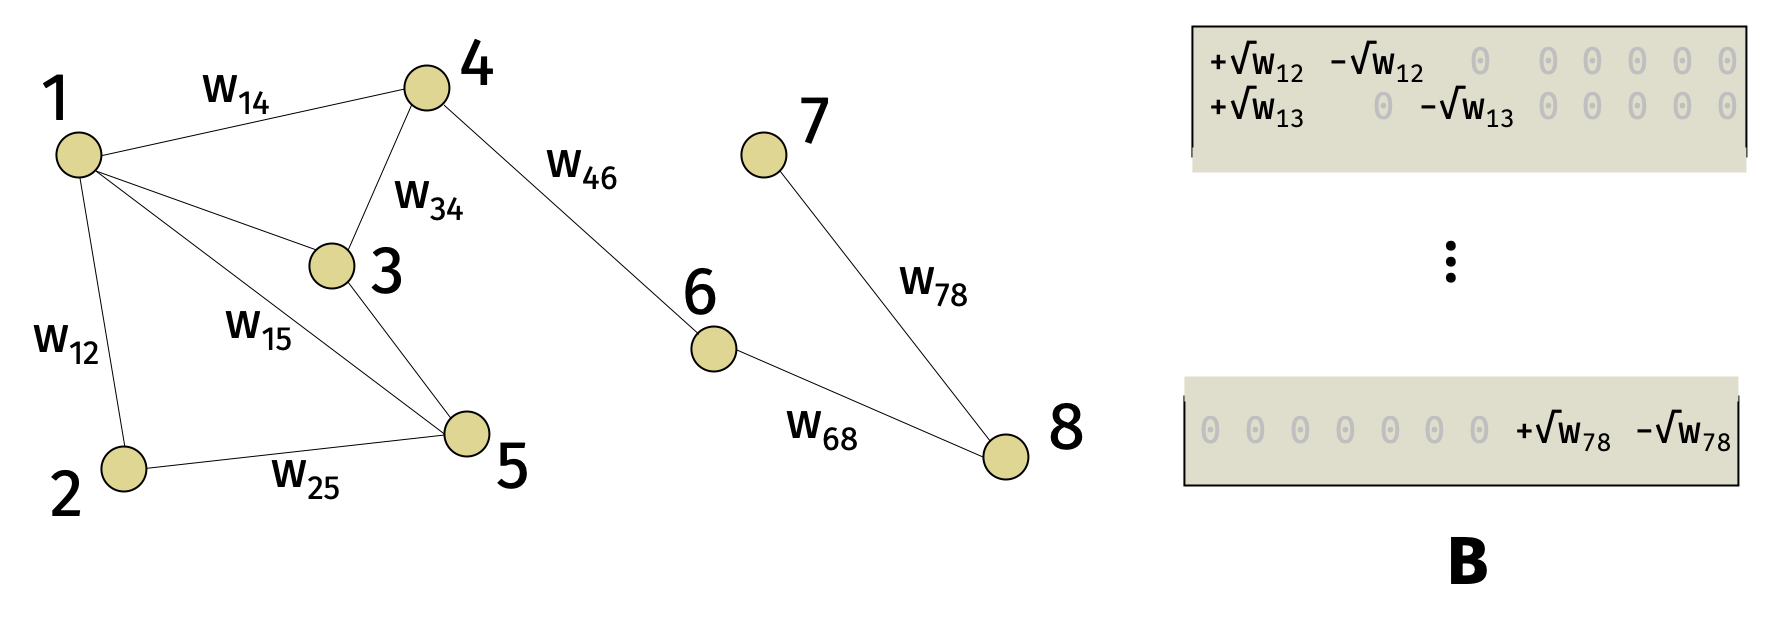
\includegraphics[width=\textwidth]{weighted_edge_vertex.png}
	\end{center}
	\vspace{-1em}
	
	And still have that if $\bv{x}\in \{-1,1\}^d$ is the \emph{cut indicator vector} for a cut $S$ in the graph, then $\frac{1}{4}\|\bv{B}\bv{x}\|_2^2 = \cut(S,V\setminus S)$.	
\end{frame}

\begin{frame}
	\frametitle{spectral sparsification}
	\textbf{Goal:} Approximate $\bv{B}$ by a weighted subsample. I.e. by $\tilde{\bv{B}}$ with $m \ll |E|$ rows, each of which is a scaled copy of a row from $\bv{B}$. 
	\begin{center}
		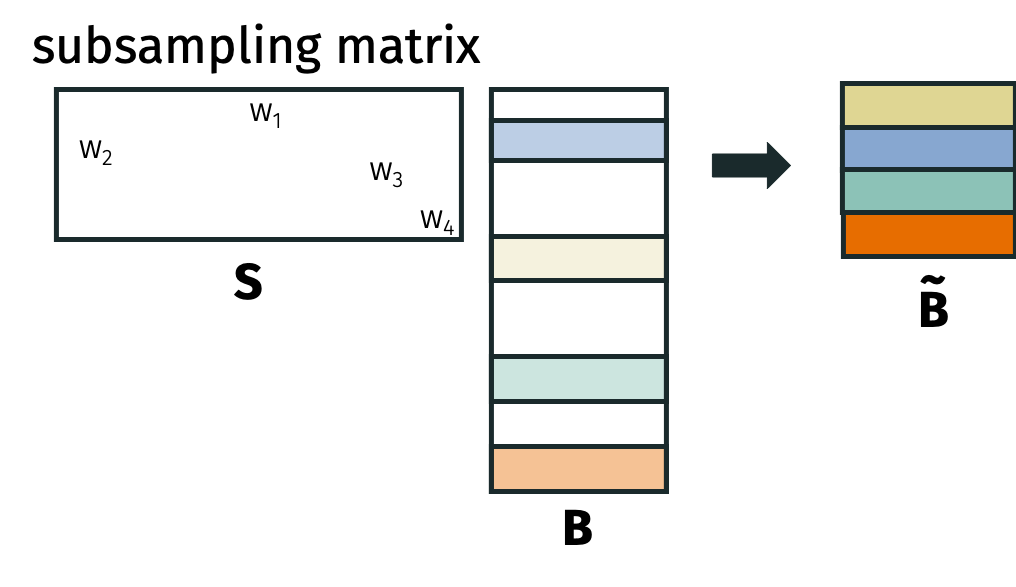
\includegraphics[width=.6\textwidth]{subsampled_b.png}
	\end{center}
	\textbf{Natural goal:} $\tilde{\bv{B}}$ is a subspace embedding for $\bv{B}$. In other words, $\tilde{\bv{B}}$ has $\approx O(d)$ rows and for all $\bv{x}$,
	\begin{align*}
		(1-\epsilon)\|\bv{B}\bv{x}\|_2^2 \leq \|\tilde{\bv{B}}\bv{x}\|_2^2 \leq (1+\epsilon)\|\bv{B}\bv{x}\|_2^2.
	\end{align*} 
\end{frame}

\begin{frame}
	\frametitle{history spectral sparsification}
	$\tilde{\bv{B}}$ is itself an edge-vertex incidence matrix for some 
	\emph{sparser} graph $\tilde{G}$!  $\tilde{G}$ is called a \emph{spectral sparsifier} for $G$.
	\vspace{-1em}
	
	\begin{center}
		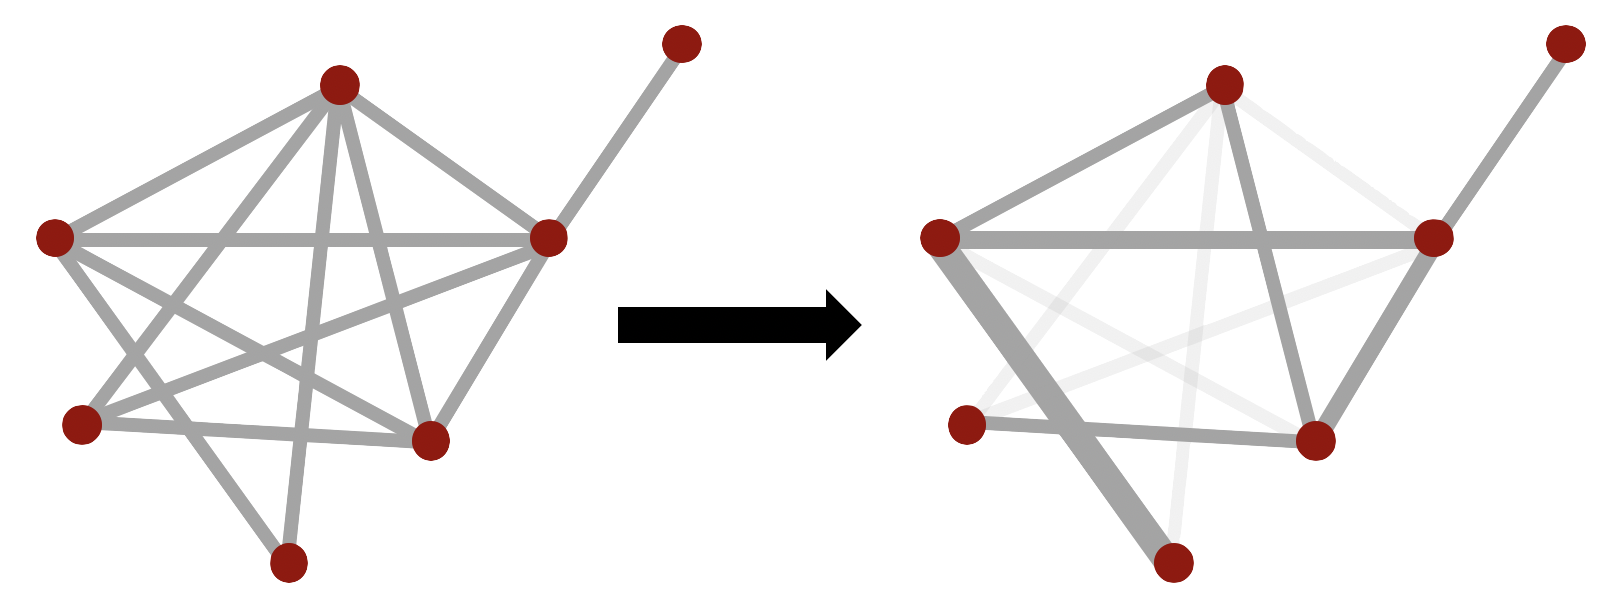
\includegraphics[width=.6\textwidth]{sparsifier.png}
	\end{center}
	
	\vspace{-1em}
	For example, we have that for any set $S$, 
	\begin{align*}
		(1-\epsilon)\cut_{{G}}(S,V\setminus S) \leq \cut_{\tilde{G}}(S,V\setminus S) \leq (1+\epsilon)\cut_{{G}}(S,V\setminus S).
	\end{align*}
	So $\tilde{G}$ can be used in place of $G$ in solving e.g. max/min cut problems, balanced cut problems, etc. 
	
	\vspace{-1em}
	\begin{center}
		\alert{In contrast $\bs{\Pi} \bv{B}$ would look nothing like an edge-vertex incidence matrix if $\bs{\Pi}$ is a JL matrix. }
	\end{center}
\end{frame}


\begin{frame}[t]
	\frametitle{history of spectral sparsification}
	Spectral sparsifiers were introduced in 2004 by Spielman and Teng in an influential paper on faster algorithms for solving Laplacian linear systems. 
	\begin{itemize}
		\item Generalize the cut sparsifiers of Benczur, Karger `96. 
		\item Further developed in work by Spielman, Srivastava + Batson, `08.
		\item Have had huge influence in algorithms, and other areas of mathematics -- this line of work lead to the 2013 resolution of the Kadison-Singer problem in functional analysis by Marcus, Spielman, Srivastava. 
	\end{itemize}
	\alert{\textbf{Rest of class}: Learn about an important random sampling algorithm for constructing spectral sparsifiers, and subspace embeddings for matrices more generally.}
\end{frame}

\begin{frame}[t]
	\frametitle{another application: active regression}	
	In many applications, computational costs are second order to \emph{data collection costs.} We have a huge range of possible data points $\bv{a}_1, \ldots, \bv{a}_n$ that we can collect labels/values $b_1,\ldots, b_n$ for. Goal is to learn $\bv{x}$ such that:
	\begin{align*}
		\bv{a}_i^T\bv{x} \approx b_i.
	\end{align*}
	Want to do so after observing as few $b_1, \ldots, b_n$ as possible. 
	Applications include healthcare, environmental science, etc. 
	\begin{center}
		\vspace{-.5em}
		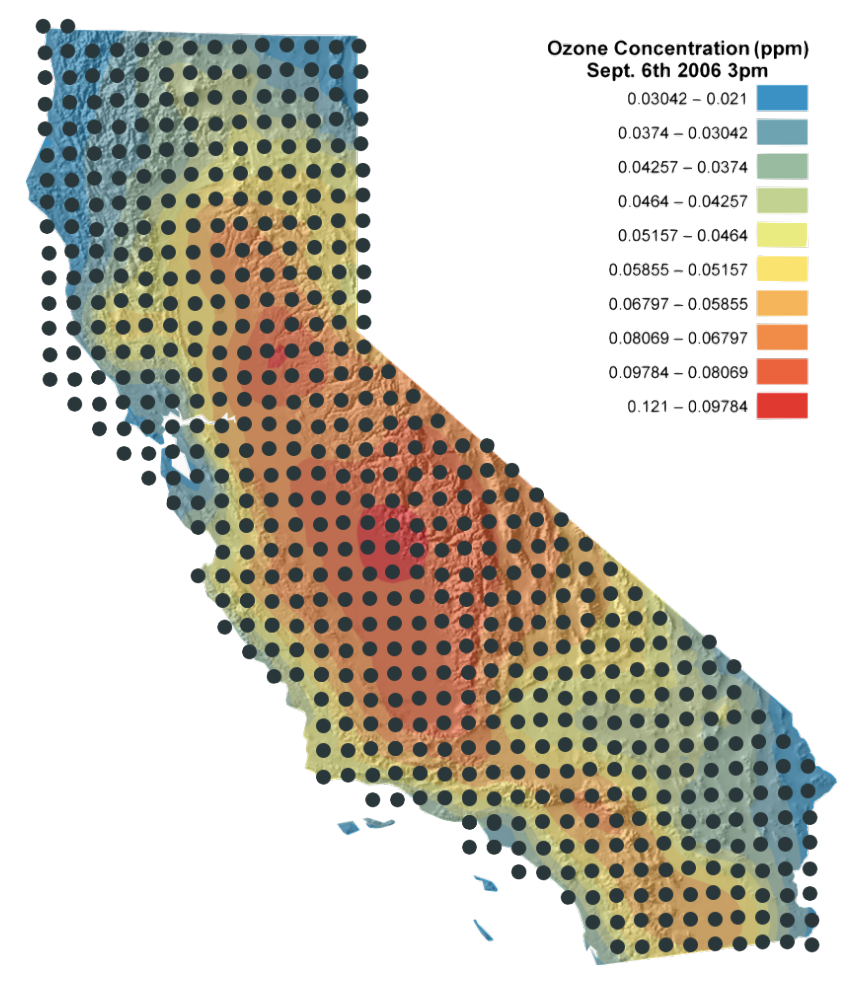
\includegraphics[width=.3\textwidth]{cali.png}
	\end{center}
\end{frame}	

\begin{frame}[t]
	\frametitle{another application: active regression}	
	\begin{itemize}
		\item Tons of applications in computational science (e.g. we have a DOE award on learning based methods for parametric PDEs). 
		\item How you collect samples really matters!
	\end{itemize}
	\begin{center}
		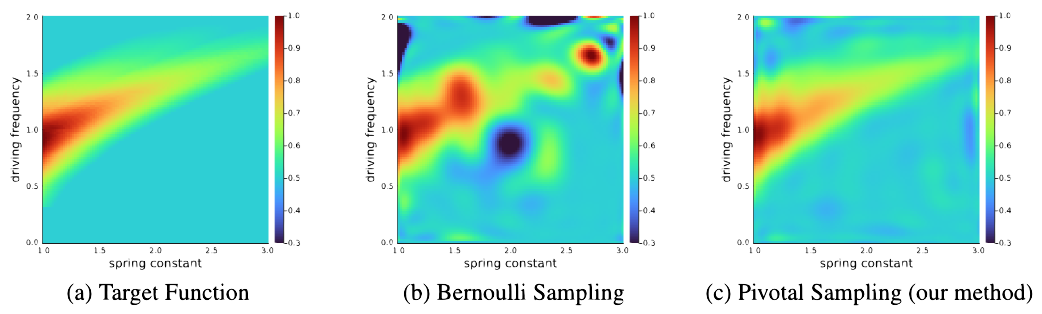
\includegraphics[width=\textwidth]{iclr_paper.png}
	\end{center}
\end{frame}

\begin{frame}[t]
	\frametitle{another application: active regression}	
	\textbf{Can be solved via random sampling} for linear models.
	\begin{center}
		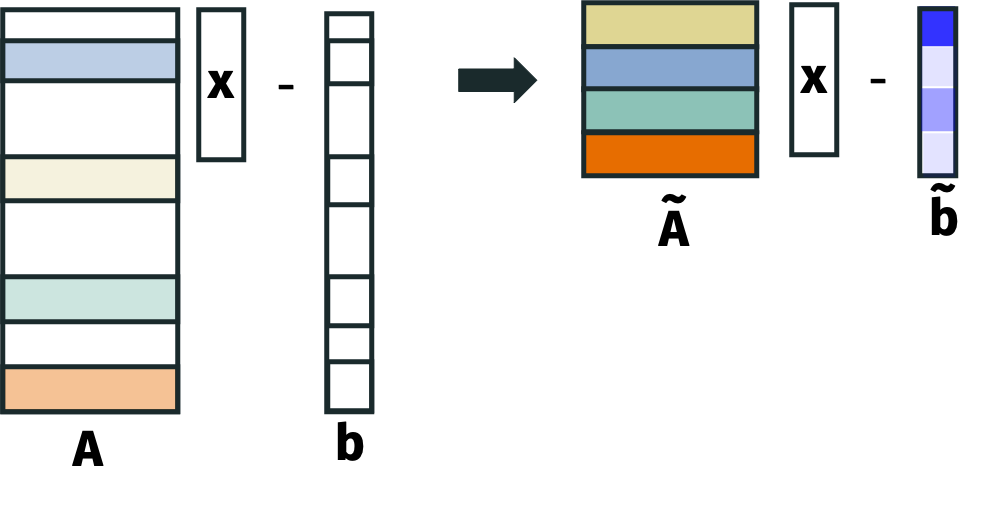
\includegraphics[width=.6\textwidth]{active_regression.png}
	\end{center}

	\textbf{Claim:} Let $\tilde{\bv{A}}$ is an $O(1)$-factor subspace embedding for $\bv{A}$ (obtained via leverage score sampling). Then $\tilde{\bv{x}} = \argmin \|\tilde{\bv{A}}\bv{x} - \tilde{\bv{b}}\|_2^2$ satisfies:
\begin{align*}
	\|\bv{A}\tilde{\bv{x}} - \bv{b}\|_2^2 \leq O(1) \|\bv{A}\bv{x}^* - \bv{b}\|_2^2, 
\end{align*}
Computing $\tilde{\bv{x}}$ only requires collecting $\tilde{O}(d)$ labels!
\end{frame}	



\begin{frame}[t]
	\frametitle{natural first attempt}
	\textbf{Goal:} Find $\tilde{\bv{A}}$ such that $\|\tilde{\bv{A}}\bv{x}\|_2^2 = (1\pm \epsilon)\|{\bv{A}}\bv{x}\|_2^2$ for all $\bv{x}$. 
	
	\textbf{Possible Approach:} Construct ${\tilde{\bv{A}}}$ by \emph{uniformly sampling} rows from $\bv{A}$. 
	
	\vspace{-2.5em}
	\begin{center}
		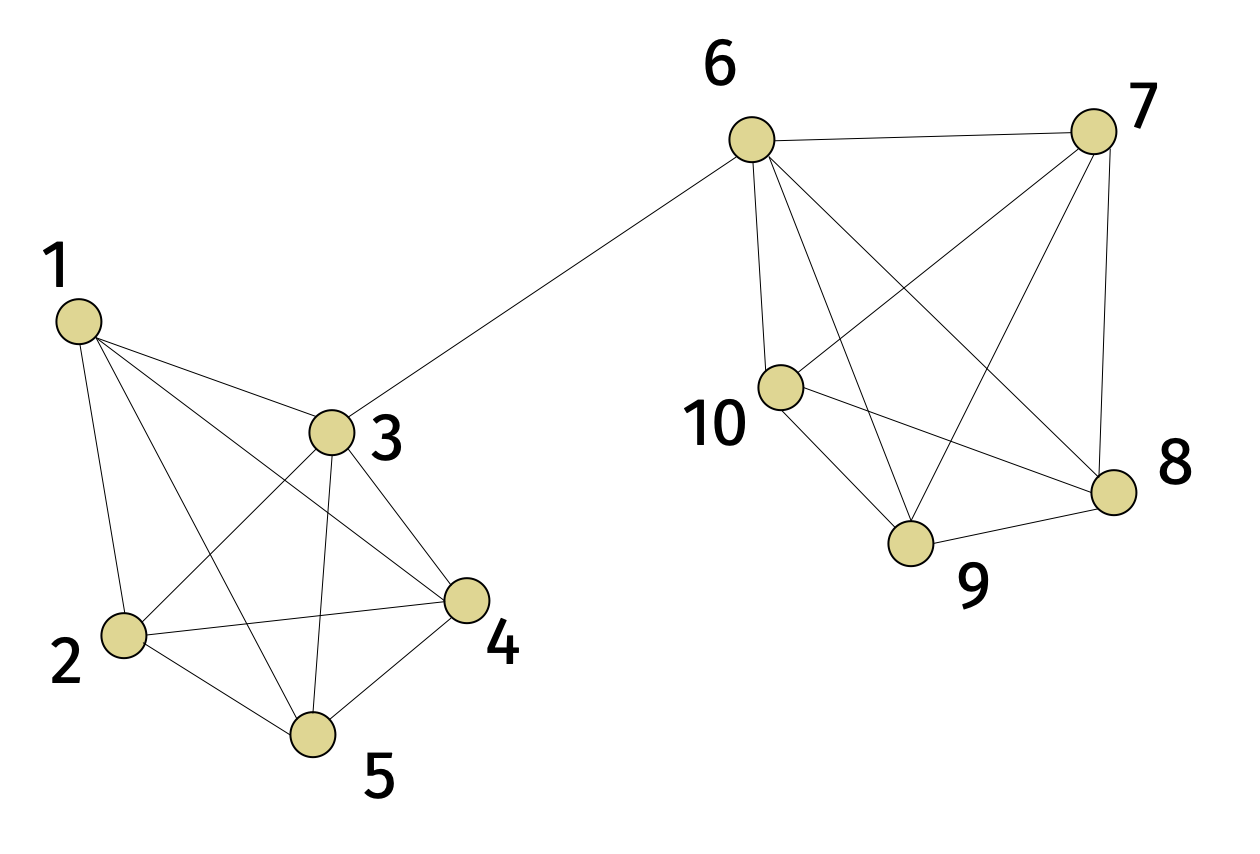
\includegraphics[width=.8\textwidth]{barbell.png}
		
		\vspace{-1.5em}
		Can check that this approach fails even for the special case of a graph vertex-edge incidence matrix. 
	\end{center}	
\end{frame}

\begin{frame}[t]
	\frametitle{importance sampling framework}
	\textbf{Key idea:} \emph{Importance sampling}. Select some rows with higher probability. 
	
	Suppose $\bv{A}$ has $n$ rows $\bv{a}_1\ldots, \bv{a}_n$. Let $p_1, \ldots, p_n \in [0,1]$ be sampling probabilities. Construct $\tilde{\bv{A}}$ as follows:
	\begin{itemize}
		\item For $i = 1,\ldots, n$
		\begin{itemize}
			\item Select $\bv{a}_i$ with probability $p_i$. 
			\item If $\bv{a}_i$ is selected, add the scaled row $\frac{1}{\sqrt{p_i}} \bv{a}_i$ to $\tilde{\bv{A}}$. 
		\end{itemize}
	\end{itemize}
	Remember, ultimately want that $\|\tilde{\bv{A}}\bv{x}\|_2^2 = (1\pm \epsilon)\|{\bv{A}}\bv{x}\|_2^2$ for all $\bv{x}$. 
	
	\textbf{Claim 1:} $\E[\|\tilde{\bv{A}}\bv{x}\|_2^2] = \|{\bv{A}}\bv{x}\|_2^2$. 
	\vspace{2em}
	
	
	\textbf{Claim 2:} Expected number of rows in $\tilde{\bv{A}}$ is $\sum_{i=1}^n p_i$. 
\end{frame}

\begin{frame}[t]
	\frametitle{lecture outline}
	\begin{center}
		\alert{\textbf{How should we choose the probabilities $p_1, \ldots, p_n$?}}
	\end{center}
\end{frame}

\begin{frame}[t]
	\frametitle{main result}
	For $i = 1, \ldots, n$, define the \emph{statistical leverage score} as:
	\begin{align*}
		\tau_i = \bv{a}_i^T(\bv{A}^T\bv{A})^{-1}\bv{a}_i.
	\end{align*}	
	\begin{theorem}[Subspace Embedding from Subsampling]
		For each $i$, and fixed constant $c$, let $p_i = \min\left(1,\frac{c\log d}{\epsilon^2}\cdot \tau_i\right)$.
		Let ${\tilde{\bv{A}}}$ have rows sampled from $\bv{A}$ with probabilities $p_1, \ldots, p_n$. With probability $9/10$, 
		\begin{align*}
			(1-\epsilon)\|\bv{A}\bv{x}\|_2^2 \leq \|\tilde{\bv{A}} \bv{x}\|_2^2 \leq	(1+\epsilon)\|\bv{A}\bv{x}\|_2^2,
		\end{align*}
		and ${\tilde{\bv{A}}}$ has $O(d\log d/\epsilon^2)$ rows in expectation. 
	\end{theorem}
\end{frame}


\begin{frame}[t]
	\frametitle{vector sampling}
	\begin{center}
		How should we choose the probabilities $p_1, \ldots, p_n$?
	\end{center}
	As usual, consider a single vector $\bv{x}$ and understand how to sample to preserve norm of $\bv{y} = \bv{A}\bv{x}$:
	\begin{align*}
		\|\tilde{\bv{A}}\bv{x}\|_2^2 = \|\bv{S}{\bv{A}}\bv{x}\|_2^2 = \|\bv{S}\bv{y}\|_2^2 \approx \|\bv{y}\|_2^2 = \|\bv{Ax}\|_2^2. 
	\end{align*}
	Then we can union bound over an $\epsilon$-net to extend to all $\bv{x}$. 
\end{frame}

\begin{frame}[t]
	\frametitle{vector sampling}
	As discussed a few lectures ago, uniform sampling only works well if $\bv{y} = \bv{A}\bv{x}$ is ``flat''. 
	\vspace{-.5em}
	\begin{center}
		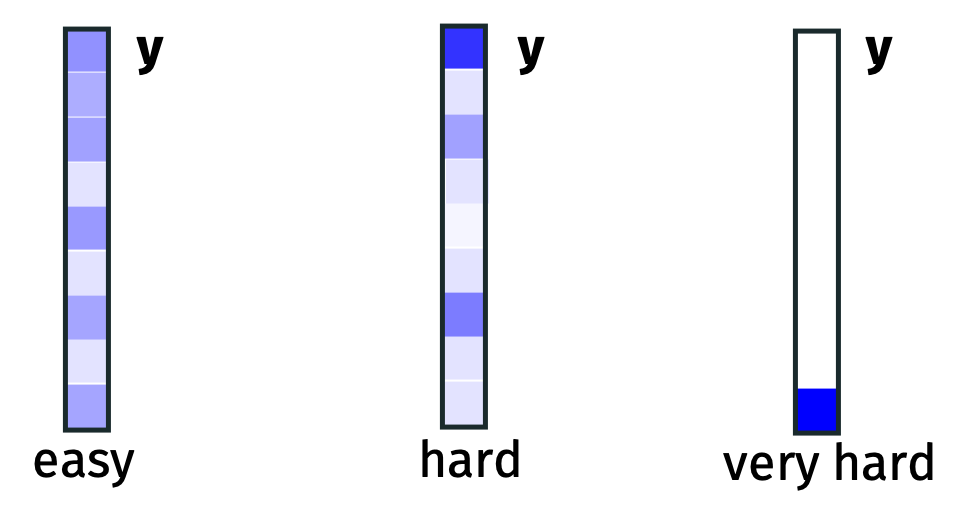
\includegraphics[width=.6\textwidth]{uniform_hard.png}
	\end{center}
	\vspace{-.5em}
	
	Instead consider sampling with probabilities at least \emph{proportional to the magnitude of $\bv{y}$'s entries}:
	\begin{align*}
		p_i > c\cdot \frac{y_i^2}{\|\bv{y}\|_2^2} \text{ for constant $c$ to be determined.}
	\end{align*}
\end{frame}

%\begin{frame}[t]
%	\frametitle{variance analysis}	
%	Let $\tilde{\bv{y}}$ be the subsampled $\bv{y}$. Recall that, when sampling with probabilities $p_1, \ldots, p_n$, for $i = 1,\ldots, n$ we add $y_i$ to $\tilde{\bv{y}}$ with probability $p_i$ and reweight by $\frac{1}{\sqrt{p_i}}$. 
%	
%	\begin{align*}
%		\|\tilde{\bv{y}}\|_2^2 &= \sum_{i=1}^n \frac{y_i^2}{p_i}\cdot Z_i & &\text{where} & Z_i&= \begin{cases}
%		1 \text{ with probability $p_i$}\\
%	0 \text{ otherwise}\end{cases}
%	\end{align*}
%	
%	\begin{align*}
%	\Var[\|\tilde{\bv{y}}\|_2^2] =  \sum_{i=1}^n \frac{y_i^2}{p_i}\cdot \Var[Z_i] \leq  \sum_{i=1}^n \frac{y_i^4}{p_i^2}\cdot p_i = \frac{y_i^4}{p_i}
%	\end{align*}
%
%We set $p_i =  c\cdot \frac{y_i^2}{\|y\|_2^2}$ so get total variance:
%\begin{align*}
%	\frac{1}{c}\|y\|_2^4
%\end{align*}
%\end{frame}	

\begin{frame}[t]
	\frametitle{variance analysis}	
	Using a Bernstein bound (or Chebyshev's inequality if you don't care about the $\delta$ dependence) we have that if $c = \frac{\log(1/\delta)}{\epsilon^2}$ then:
	\begin{align*}
			\Pr[\left|\|\tilde{\bv{y}}\|_2^2 - \|\bv{y}\|_2^2\right| \geq \epsilon \|\bv{y}\|_2^2] \leq \delta.
	\end{align*}
	
	\vspace{4em}
	The number of samples we take in expectation is:
	\begin{align*}
		\sum_{i=1}^n p_i = \sum_{i=1}^n c\cdot \frac{y_i^2}{\|\bv{y}\|_2^2} = \frac{\log(1/\delta)}{\epsilon^2}. 
	\end{align*}
\end{frame}

\begin{frame}[t]
	\frametitle{major caveat!}	
	We don't know $y_1, \ldots, y_n$! And in fact, these values aren't fixed. We wanted to prove a bound for $\bv{y} = \bv{A}\bv{x}$ for \emph{any} $\bv{x}$. 
	
	\textbf{Idea behind leverage scores:} Sample row $i$ from $\bv{A}$ using the \emph{worst case} (largest necessary) sampling probability:
	\begin{align*}
		\tau_i &= \max_{\bv{x}} \frac{y_i^2}{\|\bv{y}\|_2^2} &&\text{where} & \bv{y} = \bv{A}\bv{x}. 
	\end{align*}
	If we sample with probability $p_i = \frac{1}{\epsilon^2}\cdot \tau_i$, then we will be sampling by at least $\frac{1}{\epsilon^2}\cdot\frac{y_i^2}{\|\bv{y}\|_2^2}$, \emph{no matter what $\bv{y}$ is}. 
\end{frame}	


\begin{frame}[t]
	\frametitle{closed form expression for leverage scores}
	\begin{align*}
		\tau_i &= \max_{\bv{x}} \frac{y_i^2}{\|\bv{y}\|_2^2} &&\text{where} & \bv{y} = \bv{A}\bv{x}. 
	\end{align*}
A little messy algebra shows that $\bv{x}^* = (\bv{A}^T\bv{A})^{-1}\bv{a}_i$.
\end{frame}

\begin{frame}[t]
	\frametitle{leverage score sampling}
	\textbf{Leverage score sampling:}
	\begin{itemize}
		\item For $i = 1, \ldots, n$, 
		\begin{itemize}
			\item Compute $\tau_i = \bv{a}_i^T(\bv{A}^T\bv{A})^{-1}\bv{a}_i$. 
			\item Set $p_i = \frac{c\log(1/\delta)}{\epsilon^2}\cdot \tau_i$.
			\item Add row $\bv{a}_i$ to $\tilde{\bv{A}}$ with probability $p_i$ and reweight by $\frac{1}{\sqrt{p_i}}$.  			
		\end{itemize}
	\end{itemize}
	For any fixed $\bv{x}$, we will have that $(1-\epsilon) \|{\bv{A}}\bv{x}\|_2^2\leq \|\tilde{\bv{A}}\bv{x}\|_2^2 \leq (1+\epsilon) \|{\bv{A}}\bv{x}\|_2^2$ with probability $(1-\delta)$. 
	
	\textbf{Two remaining concerns:}
	
	1) How do we extend from \emph{any} $\bv{x}$ to \emph{all} $\bv{x}$?
	
	2) The number of samples we take will be roughly $\sum_{i=1}^n \tau_i$. How do we bound this?
\end{frame}


\begin{frame}[t]
	\frametitle{sum of leverage scores}
	\textbf{Claim:} No matter how large $n$ is, $\sum_{i=1}^n \tau_i = d$ for a matrix $\bv{A}\in \R^d$. 
	
	
	\vspace{12em}
	\begin{center}
		\alert{``Zero-sum'' law for the importance of matrix rows.}
	\end{center}
\end{frame}


\begin{frame}[t]
	\frametitle{main result}
	Naive $\epsilon$-net argument leads to $d^2$ dependence since we need to set $\delta = c^d$. Getting the right $d\log d$ dependence below requires a standard ``matrix Chernoff bound'' (see e.g. Tropp 2015). 
	\begin{theorem}[Subspace Embedding from Subsampling]
		For each $i$, and fixed constant $c$, let $p_i = \min\left(1,\frac{c\log d}{\epsilon^2}\cdot \tau_i\right)$.
		Let ${\tilde{\bv{A}}}$ have rows sampled from $\bv{A}$ with probabilities $p_1, \ldots, p_n$. With probability $9/10$, 
		\begin{align*}
			(1-\epsilon)\|\bv{A}\bv{x}\|_2^2 \leq \|\tilde{\bv{A}} \bv{x}\|_2^2 \leq	(1+\epsilon)\|\bv{A}\bv{x}\|_2^2,
		\end{align*}
		and ${\tilde{\bv{A}}}$ has $O(d\log d/\epsilon^2)$ rows in expectation. 
	\end{theorem}
\end{frame}

\begin{frame}[t]
	\frametitle{spectral sparsification corollary}
	For any graph $G$ with $d$ nodes, there exists a graph $\tilde{G}$ with $O(d\log d/\epsilon^2)$ edges such that, for all $\bv{x}$, $\|\tilde{\bv{B}}\bv{x}\|_2^2 = (1\pm\epsilon)\|{\bv{B}}\bv{x}\|_2^2$. 
	\begin{center}
		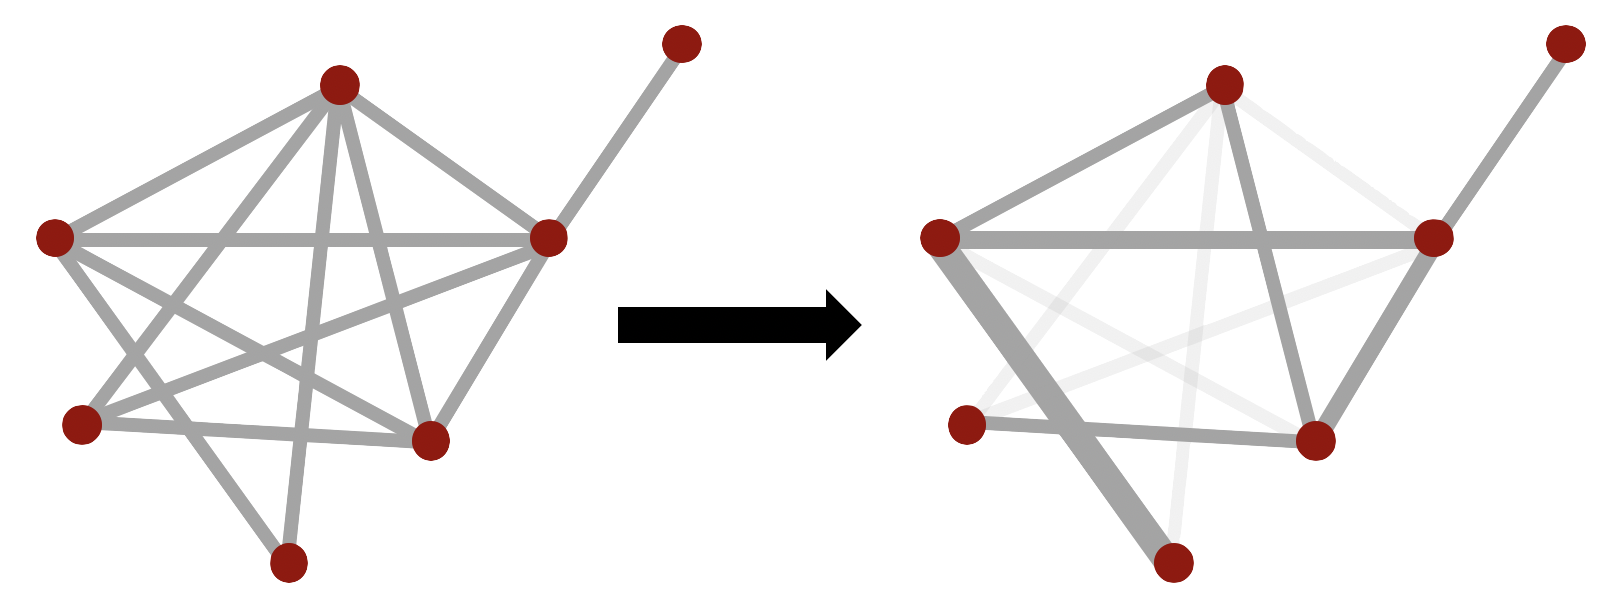
\includegraphics[width=.6\textwidth]{sparsifier.png}
	\end{center}
As a result, the value of any cut in $\tilde{G}$ is within a $(1\pm \epsilon)$ factor of the value in $G$, the Laplacian eigenvalues are with a $(1\pm \epsilon)$ factors, etc. 
\end{frame}

\begin{frame}[t]
	\frametitle{thank you!}
	Thank you all for a great course! If you are interested in learning even more, there are several seminars at NYU that you might be interested in attending:

	\textbf{Theoretical Computer Science Seminar:} \color{blue} \href{https://csefoundations.engineering.nyu.edu/seminar.html}{https://csefoundations.engineering.nyu.edu/seminar.html}.  \color{black}

	\textbf{Math and Data Seminar:} \color{blue} \href{https://mad.cds.nyu.edu/seminar/}{https://mad.cds.nyu.edu/seminar/}. \color{black}

	\textbf{Computational Math and Scientific Computing Seminar:} \color{blue} \href{https://cims.nyu.edu/dynamic/calendars/seminars/computational-mathematics-and-scientific-computing-seminar/}{https://cims.nyu.edu/dynamic/calendars/seminars/computational-mathematics-and-scientific-computing-seminar/}. \color{black}

\end{frame}
	
\end{document} 








